\chapter{Proposed Design}\label{ch:proposed-design}

\define{Risk propagation} is a message-passing algorithm that estimates an individual's infection risk by considering their demographics, symptoms, diagnosis, and contact with others. Formally, a \define{risk score} $\vScore_\vTime \in [0, 1]$ is a timestamped infection probability where $\vTime \in \naturals$ is the time of its computation. Thus, an individual with a high risk score is likely to test positive for the infection and poses a significant health risk to others. There are two types of risk scores: \define{symptom scores}, or prior infection probabilities, which account for an individual's demographics, symptoms, and diagnosis \citep{Briers2020, Menni2020}; and \define{exposure scores}, or posterior infection probabilities, which incorporate the risk of direct and indirect contact with others.

Given their recent risk scores and contacts, an individual's exposure score is derived by marginalizing over the joint infection probability distribution. Naively computing this marginalization scales exponentially with the number of variables (i.e., individuals). To circumvent this intractability, the joint distribution is modeled as a factor graph, and an efficient message-passing procedure is employed to compute the marginal probabilities with a time complexity that scales linearly in the number of factor \verticesName (i.e., contacts).

Let $\vGraph = (\vVariables, \vFactors, \vEdges)$ be a \define{factor graph} where $\vVariables$ is the set of variable \verticesName, $\vFactors$ is the set of factor \verticesName, and $\vEdges$ is the set of edges incident between them \citep{Kschischang2001}. A \define{variable \vertexName} $\vVariable: \eventSpace \rightarrow \{0, 1\} $ is a random variable that represents the infection status of an individual, where the sample space is $\eventSpace = \{\var{healthy}, \var{infected}\}$ and
\begin{equation*}
  \vVariable(\event) =
    \begin{cases}
      0 & \text{if } \event = \var{healthy} \\
      1 & \text{if } \event = \var{infected}.
    \end{cases}
\end{equation*}
Thus, $\pr{\vVariable[i]}[\vTime] = \vScore_\vTime$ is a risk score of \indexed{i}{individual}. A \define{factor \vertexName} $\vFactor: \vVariables \times \vVariables \rightarrow [0, 1]$ defines the transmission of infection risk between two contacts. Specifically, contact between \twoindexed{i}{j}{individual} is represented by the factor \vertexName $\vFactor(\vVariable[i], \vVariable[j])$ = $\vFactor[ij]$, which is adjacent to the variable \verticesName $\vVariable[i], \vVariable[j]$. \Cref{fig:factor-graph} depicts a factor graph that reflects the domain constraints.

\begin{figure}[htbp]
\centering
\begin{tikzpicture}[ampersand replacement=\&]
  \matrix[row sep=1.5em, column sep=0.75em] {
    \& \factor[minimum size=1em] {f12} {above:$\vFactor[12]$} {} {}; \&\&
    \factor[minimum size=1em] {f23} {above:$\vFactor[23]$} {} {}; \& \\
    \node[latent, minimum size=2em] (v1) {$\vVariable[1]$}; \&\&
    \node[latent, minimum size=2em] (v2) {$\vVariable[2]$}; \&\&
    \node[latent, minimum size=2em] (v3) {$\vVariable[3]$}; \\
  };
  \edge[-] {v1} {f12};
  \edge[-] {v2} {f12};
  \edge[-] {v2} {f23};
  \edge[-] {v3} {f23};
\end{tikzpicture}
\caption[Factor graph]{A factor graph of 3 variable \verticesName and 2 factor \verticesName.}
\label{fig:factor-graph}
\end{figure}

\section{Synchronous Risk Propagation}\label{sec:synchronous}

\citet{Ayday2021} first proposed risk propagation as a synchronous, iterative message-passing algorithm that uses the factor graph to compute exposure scores. The first input to \cRiskPropagation is the set family $\vScores$, where
\begin{equation} \label{eq:score-set}
  \vScores_i =\setBuilder{\vScore_t}{\vReferenceTime - \vTime < \pScoreExpiry} \in \vScores
\end{equation}
is the set of recent risk scores of \indexed{i}{individual}. The second input to \cRiskPropagation is the contact set
\begin{equation} \label{eq:contact-set}
  \vContacts = \setBuilder{(i, j, \vTime)}{i \neq j, \vReferenceTime - \vTime < \pContactExpiry}
\end{equation}
such that $(i, j, \vTime)$ is the \emph{most recent} contact between \twoindexed{i}{j}{individual} that occurred from time $\vTime$ until at least time $\vTime + \pMinContactDuration$, where $\pMinContactDuration \in \naturals$ is the \define{minimum contact duration}. Naturally, risk scores and contacts have finite relevance, so \cref{eq:score-set,eq:contact-set} are constrained by the \define{risk score expiry} $\pScoreExpiry \in \naturals$ and the \define{contact expiry} $\pContactExpiry \in \naturals$, respectively. The \define{reference time} $\vReferenceTime \in \naturals$ defines the relevance of the inputs and is assumed to be the time at which \cRiskPropagation is invoked. For notational simplicity in \cRiskPropagation, let $\vSomeSet$ be a set. Then $\max \vSomeSet = 0$ if $\vSomeSet = \emptyset$.

\subsection{Variable Messages}

The current exposure score of \indexed{i}{individual} is defined as $\max \vScores_i$. Hence, a \define{variable message} $\vVariableMessage{i}{j}{n}$ from the variable \vertexName $\vVariable[i]$ to the factor \vertexName $\vFactor[ij]$ during \indexed{n}{iteration} is the set of maximal risk scores $\vRiskScores{i}{n - 1}$ from the previous $n - 1$ iterations that were not derived by $\vFactor[ij]$. In this way, risk propagation is reminiscent of the max-sum algorithm; however, risk propagation aims to maximize \emph{individual} marginal probabilities rather than the joint distribution \citep[pp. 411--415]{Bishop2006}.

\subsection{Factor Messages}

A \define{factor message} $\vFactorMessage{i}{j}{n}$ from the factor \vertexName $\vFactor[ij]$ to the variable \vertexName $\vVariable[j]$ during \indexed{n}{iteration} is an exposure score of \indexed{j}{individual} that is based on interacting with those at most $n - 1$ degrees separated from \indexed{i}{individual}. This population is defined by the subgraph induced in $\vGraph$ by
\begin{equation*}
  \setBuilder{\vVertex \in \vVariables \cap \vFactors \setminus \{\vVariable[j], \vFactor[ij]\}}{\dist(\vVariable[i], \vVertex) \leq 2(n - 1)},
\end{equation*}
where $\dist(\vSourceVertex, \vTargetVertex)$ is the shortest-path distance between the \verticesName $\vSourceVertex, \vTargetVertex$. The computation of a factor message assumes the following.
\begin{enumerate}
  \item Contacts have a nondecreasing effect on an individual's exposure score.
  \item A risk score $\vScore_\vTime$ is \define{relevant} to the contact $(i, j, \vTime_{ij})$ if $\vTime < \vTime_{ij} +\pTimeBuffer$, where $\pTimeBuffer \in \naturals$ is a \define{time buffer} that accounts for the incubation period, along with the delayed reporting of symptom scores and contacts. The time buffer is also known as the \define{(contact) tracing window} \citep{Raymenants2022} and is similar to the \define{notification window} used by other contact tracing applications \citep{Leng2022}.
  \item Risk transmission between contacts is incomplete. Thus, a risk score decays exponentially along its transmission path in $\vGraph$ at a rate of $\log \pTransmissionRate$, where $\pTransmissionRate \in (0, 1)$ is the \define{transmission rate}. \Cref{fig:decay} visualizes this decay, assuming a transmission rate of $\pTransmissionRate = 0.8$ \citep{Hamner2020}.\end{enumerate}

\begin{figure}[htbp]
\centering
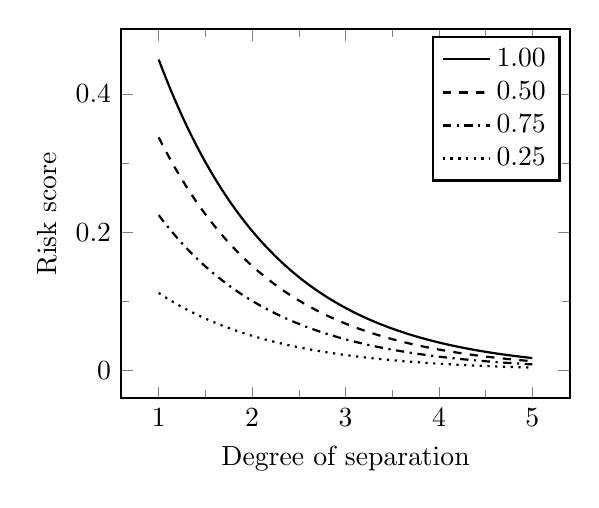
\begin{tikzpicture}
\begin{axis}[
  xlabel={Degree of separation},
  ylabel={Risk score},
  minor tick num=1,
  width=0.6\textwidth,
  smooth,
  domain=1:5,
  y domain=0.01:1,
  samples=100,
  black,
  thick
]
  \addplot[] {e^(-0.8 * x)};
  \addplot[dashed] {0.75 * e^(-0.8 * x)};
  \addplot[dashdotted] {0.5 * e^(-0.8 * x)};
  \addplot[dotted] {0.25 * e^(-0.8 * x)};
  \legend{$1.00$, $0.50$, $0.75$, $0.25$};
\end{axis}
\end{tikzpicture}
\caption[Exponential decay of risk scores]{Exponential decay of risk scores.}
\label{fig:decay}
\end{figure}

To reiterate, a factor message $\vFactorMessage{i}{j}{n}$ is the maximum relevant risk score in the variable message $\vVariableMessage{i}{j}{n}$ (or 0) that is scaled by the transmission rate $\pTransmissionRate$.

\citet{Ayday2021} assume that the contact set $\vContacts$ may contain (1) multiple contacts between the same two individuals and (2) invalid contacts, or those lasting less than $\pMinContactDuration$ time. However, these assumptions introduce unnecessary complexity. Regarding assumption 1, suppose \twoindexed{i}{j}{individual} come into contact $m$ times such that $\vTime_k < \vTime_\ell$ for $1 \leq k < \ell \leq m$. Let $\vFactorMessages_k$ be the set of relevant risk scores, according to the contact time $\vTime_k$, where
\begin{equation*}
  \vFactorMessages_k = \setBuilder{\pTransmissionRate \vScore_t}{\vScore_\vTime \in \vVariableMessage{i}{j}{n}, \vTime < \vTime_k + \pTimeBuffer}.
\end{equation*}
Then $\vFactorMessages_k \subseteq \vFactorMessages_\ell$ if and only if $\max \vFactorMessages_k \leq \max \vFactorMessages_\ell$. Therefore, only the most recent contact time $t_m$ is required to compute the factor message $\vFactorMessage{i}{j}{n}$. With respect to assumption 2, there are two possibilities.
\begin{enumerate}
  \item If an individual has at least one valid contact, then their exposure score is computed over the subgraph induced in $\vGraph$ by their contacts that define the neighborhood $\vNeighbors_i$ of the variable \vertexName $\vVariable_i$.
  \item If an individual has no valid contacts, then their exposure score is $\max \vScores_i$ or $0$, if all of their previously computed risk scores have expired.
\end{enumerate}
In either case, a set $\vContacts$ containing only valid contacts implies fewer factor \verticesName and edges in the factor graph $\vGraph$. Consequently, the complexity of \cRiskPropagation is reduced by a constant factor since fewer messages must be computed.

\subsection{Termination}

To detect convergence, the normed difference between the current and previous exposure scores is compared to the threshold $\pDiff \in \reals$. Note that $\vExposureScores{n}$ is the vector of exposure scores in the \indexed{n}{iteration} such that $\vExposureScore{i}{n}$ is \indexed{i}{component} of $\vExposureScores{n}$. The $L_1$ and $L_\infty$ norms are sensible choices for detecting convergence. \citet{Ayday2021} use the $L_1$ norm, which ensures that an individual's exposure score changed by at most $\pDiff$ after the penultimate iteration.

\begin{function}[H]{\nRiskPropagation}[\vScores, \vContacts]
  \State $(\vVariables, \vFactors, \vEdges) \assign \cCreateFactorGraph[\vContacts]$
  \State $n \assign 1$
  \ForEach{$\vVariable[i] \in \vVariables$}
    \State $\vRiskScores{i}{n - 1} \assign \topK{\vScores_i}$
    \State $\vExposureScore{i}{n - 1} \assign \max \vRiskScores{i}{n - 1}$
    \State $\vExposureScore{i}{n} \assign \infty$
  \EndFor
  \While{$\| \vExposureScores{n} - \vExposureScores{n - 1} \| > \pDiff$}
    \ForEach{$\{\vVariable[i], \vFactor[ij]\} \in \vEdges$}
      \State $\vVariableMessage{i}{j}{n} \assign \vRiskScores{i}{n - 1} \setminus \setBuilder{\vFactorMessage{j}{i}{\ell}}{\ell \in \intInterval{1}{n - 1}}$
    \EndFor
    \ForEach{$\{\vVariable[i], \vFactor[ij]\} \in \vEdges$}
      \State $\vFactorMessage{i}{j}{n} \assign \max \setBuilder{\pTransmissionRate \vScore_\vTime}{\vScore_\vTime \in \vVariableMessage{i}{j}{n}, \vTime < \vTime_{ij} + \pTimeBuffer}$
    \EndFor
    \ForEach{$\vVariable[i] \in \vVariables$}
      \State $\vRiskScores{i}{n} \assign \topK{\setBuilder{\vFactorMessage{j}{i}{n}}{\vFactor[ij] \in \vNeighbors_i}}$
    \EndFor
    \ForEach{$\vVariable[i] \in \vVariables$}
      \State $\vExposureScore{i}{n - 1} \assign \vExposureScore{i}{n}$
      \State $\vExposureScore{i}{n} \assign \max \vRiskScores{i}{n}$
    \EndFor
    \State $n \assign n + 1$
  \EndWhile
  \State \Return $\vExposureScores{n}$
\end{function}

\section{Asynchronous Risk Propagation}\label{sec:asynchronous}

While \cRiskPropagation offers proof of concept, it is not viable for real-world application. \cRiskPropagation is an \define{offline algorithm} \citep{Cormen2022}, because it requires the contact and health information of all individuals as input. As \citet{Ayday2021} note, this centralization of personal data is not privacy-preserving. \cRiskPropagation also introduces communication overhead and computational redundancy since most exposure scores are unlikely to change across frequent invocations. To mitigate this inefficiency, \citet{Ayday2020} suggest running \cRiskPropagation once or twice per day. Unfortunately, this cadence incurs substantial delay in updating individuals' exposure scores. In the midst of a pandemic, timely information is essential for individual and collective health. 

To address the limitations of \cRiskPropagation, \citet{Ayday2021} propose decentralizing the factor graph such that the processing entity associated with \indexed{i}{individual} maintains the state of \indexed{i}{variable \vertexName} and the neighboring factor \verticesName. Applying one-mode projection onto the variable \verticesName \citep{Zhou2007}, \cref{fig:projected} illustrates how each entity corresponds to a portion of the factor graph. More generally, \citet{Ayday2021} envision risk propagation as a decentralized communication protocol for informing individuals about their infection risk. Such a message-passing protocol naturally aligns with the \define{actor model}, a local model of concurrent computing that defines computation as patterns of message passing amongst computational entities called \define{actors} \citep{Hewitt1973, Hewitt1977a, Hewitt1977b,Clinger1981, Agha1985, De_Koster2016}. Since communication is asynchronous in the actor model, risk propagation defined in this way is called \define{asynchronous risk propagation}.

\begin{figure}[htbp]
\centering
\begin{tikzpicture}[ampersand replacement=\&]
  \matrix[row sep=7em, column sep=2em] {
    \node[latent, minimum size=2em] (v1) {$\vVariable[1]$}; \&\&\&
    \node[latent, minimum size=2em] (v2) {$\vVariable[2]$}; \&\&\&
    \node[latent, minimum size=2em] (v3) {$\vVariable[3]$}; \\
  };
  \factor[minimum size=1em, above= of v1] {f12_1} {above:$\vFactor[12]$} {} {};
  \factor[minimum size=1em, above= of v2, xshift=-3em] {f12_2} {above:$\vFactor[12]$} {} {};
  \factor[minimum size=1em, above= of v2, xshift=3em] {f23_2} {above:$\vFactor[23]$} {} {};
  \factor[minimum size=1em, above= of v3] {f23_3} {above:$\vFactor[23]$} {} {};
  
  \plate{p1} {(v1)(f12_1)(f12_1-caption)} {};
  \plate{p2} {(v2)(f12_2)(f23_2)(f12_2-caption)(f23_2-caption)} {};
  \plate{p3} {(v3)(f23_3)(f23_3-caption)} {};
  
  \edge[-] {v1} {f12_1};
  \edge[-] {v2} {f12_2};
  \edge[-] {v2} {f23_2};
  \edge[-] {v3} {f23_3};
  \edge[-] {p1} {p2};
  \edge[-] {p2} {p3};
\end{tikzpicture}
\caption[One-mode projection of the factor graph]{One-mode projection onto the variable \verticesName in \cref{fig:factor-graph}.}
\label{fig:projected}
\end{figure}

\subsection{Actor Behavior}

An actor $\vActor$ in the ShareTrace actor system corresponds to an individual and is initialized by the \cCreateActor operation \citep{Agha1985} with the following attributes.
\begin{itemize}
  \item $\aActorExposure$: the current exposure score of the individual. This attribute is either a symptom score, a risk score sent by another actor, or the null risk score (see \cNullRiskScore).
  \item $\aActorContacts$: a \define{dictionary} (see \cref{ch:data-structures}) of contacts. In the context of an actor, a contact is a \define{proxy} \citep{Gamma1995} of the actor that represents an individual with which the individual represented by this actor was physically proximal. That is, if \indexed{i}{individual} interacted with \indexed{j}{individual}, then $\aContacts{\vActor_i}$ contains a contact $\vContact$ such that $\aContactKey = \aContactName$ is a name of \indexed{j}{actor} and $\aContactTime$ is the most recent time of contact. This attribute extends the concept of \define{actor acquaintances} \citep{Hewitt1977a, Hewitt1977b, Agha1985} to be time-varying.
  \item $\aActorScores$: a dictionary of exposure scores such that $\aScoreKey$ for an exposure score $\vScore$ is the time interval during which $\aActorExposure = \vScore$. The null risk score is returned for queries in which the dictionary does not contain a risk score with a key that intersects the given query interval. \Cref{fig:exposure} depicts a hypothetical step function that $\aActorScores$ represents.
\end{itemize}

\begin{function}[H]{\nNullRiskScore}
  \State $\aScoreValue \assign 0$
  \State $\aScoreTime \assign 0$
  \State \Return $\vScore$
\end{function}

\begin{function}[H]{\nCreateActor}
  \State $\aActorContacts \assign \emptyset$
  \State $\aActorScores \assign \emptyset$
  \State $\aActorExposure \assign \cNullRiskScore$
  \State \Return $\vActor$
\end{function}

\begin{figure}[htbp]
\centering
\begin{tikzpicture}
\begin{axis}[
  xlabel={Time},
  ylabel={Exposure score},
  xtick=\empty,
]
  \addplot [const plot mark right] coordinates {
    (0, 0)
    (2, 0)
    (3, 0.3)
    (6, 0.7)
    (9, 0.6)
    (11, 0.9)
    (15, 0.8)
    (17, 0.4)
  };
\end{axis}
\end{tikzpicture}
\caption[Historical exposure scores of an actor]{Hypothetical history of an individual's exposure score.}
\label{fig:exposure}
\end{figure}

The interface of an actor is primarily defined by two types of messages: contacts and risk scores. Based on \cref{sec:synchronous}, let the \define{time to live} (TTL) of a message be the remaining time of its relevance. The reference time $\vReferenceTime$ is assumed to be the current time.

\begin{function}{\nRiskScoreTtl}[\vScore]
  \State \Return $\pScoreExpiry - (\vReferenceTime - \aScoreTime)$
\end{function}

\begin{function}{\nContactTtl}[\vContact]
  \State \Return $\pContactExpiry - (\vReferenceTime - \aContactTime)$
\end{function}

The \cHandleRiskScore operation defines how an actor behaves upon receiving a risk score. The key $\aScoreKey$ initially associated with the risk score $\vScore$ is the time interval during which it is relevant. For the dictionary $\aActorScores$, \cMerge preserves the mapping invariant defined above such that risk scores are ordered first by value and then by time. Thus, $\aScoreKey \subseteq [\aScoreTime, \aScoreTime + \pScoreExpiry)$ for all exposure scores in $\aActorScores$. The \cUpdateExposureScore operation is the online equivalent of updating an individual's exposure score in \cRiskPropagation.

\begin{function}[H]{\nHandleRiskScore}[\vActor, \vScore]
  \If{$\cRiskScoreTtl[\vScore] > 0$}
    \State $\aScoreKey \assign [\aScoreTime, \aScoreTime + \pScoreExpiry)$
    \State $\cMerge[\aActorScores, \vScore]$
    \State $\cUpdateExposureScore[\vActor, \vScore]$
    \ForEach{$\vContact \in \aActorContacts$}
      \State $\cApplyRiskScore[\vActor, \vContact, \vScore]$
    \EndFor
  \EndIf
\end{function}

\begin{function}[H]{\nUpdateExposureScore}[\vActor, \vScore]
  \If{$\aActorExposureValue < \aScoreValue$}
    \State $\aActorExposure \assign \vScore$
  \ElsIf{$\cRiskScoreTtl[\aActorExposure] \leq 0$}
    \State $\aActorExposure \assign \cMaximum[\aActorScores]$
  \EndIf
\end{function}

For the moment, assume that \cApplyRiskScore is the online equivalent of computing a factor message (see \cref{sec:synchronous}). Line \ref{step:scale-by-transmission-rate} indicates that a copy $\vNewScore$ of the risk score $\vScore$ is updated using the transmission rate $\pTransmissionRate$. The \cSend operation enables actor communication \citep{Agha1985}.

\begin{function}[H]{\nApplyRiskScore}[\vActor, \vContact, \vScore]
  \If{$\aContactTime + \pTimeBuffer > \aScoreTime$}
    \State $\aNewScoreValue \assign \pTransmissionRate \cdot \aScoreValue$ \label{step:scale-by-transmission-rate}
    \State $\cSend[\aContactName, \vNewScore]$
  \EndIf
\end{function}

The problem with \cApplyRiskScore is that it causes risk scores to propagate \textit{ad infinitum}. Unlike \cRiskPropagation, a global convergence test is not available to terminate message passing, so it is necessary to define a local condition that determines if a risk score should be sent to another actor. Practically, ``self-terminating'' message-passing is necessary for asynchronous risk propagation to be scalable and cost-efficient.

The intent of sending a risk score to an actor is to update its exposure score. According to \cHandleRiskScore, it is only necessary to send an actor risk scores with values that exceed its current exposure score. Thus, an actor can associate a \define{send threshold} with a contact such that the target actor only receives risk scores that exceed the threshold. To permit a trade-off between accuracy and efficiency, let the \define{send coefficient} $\pSendCoefficient \in \reals$ and \define{tolerance} $\pTolerance \in \reals$ be scaling factors that are applied to a risk score upon setting the send threshold.

\begin{function}{\nSetSendThreshold}[\vContact, \vScore]
  \State $\aNewScoreValue \assign \pSendCoefficient \cdot \aScoreValue + \pTolerance$
  \State $\aContactThreshold \assign \vNewScore$
\end{function}

The \cApplyRiskScore operation that incorporates the concept of a send threshold is defined below. Assuming a finite number of actors, a positive send coefficient guarantees that a risk score has finite propagation.

\begin{function}{\nApplyRiskScore}[\vActor, \vContact, \vScore]
  \If{$\aContactThresholdValue < \aScoreValue \AND \aContactTime + \pTimeBuffer > \aScoreTime$}
    \State $\aNewScoreValue \assign \pTransmissionRate \cdot \aScoreValue$
    \State $\cSetSendThreshold[\vContact, \vNewScore]$
    \State $\cSend[\aContactName, \vNewScore]$
  \EndIf
\end{function}

The \cSetSendThreshold operation defines \emph{how} the send threshold is updated, but not \emph{when} it should be updated; the \cUpdateSendThreshold operation encapsulates the latter. The second predicate on Line \ref{step:should-update-threshold} stems from the fact that the send threshold is a risk score and thus subject to expiry. The first predicate, however, is more subtle and will be revisited shortly. The \cMaximumOlderThan operation is the same as \cMaximum, with the constraint that the key of the risk score intersects the interval $(-\infty, \aContactTime + \pTimeBuffer)$. Thus, the returned risk score is always relevant to the contact. Consistent with \cApplyRiskScore, the risk score retrieved from $\aActorScores$ is scaled by the transmission rate and set as the new send threshold.

\begin{function}{\nUpdateSendThreshold}[\vActor, \vContact]
  \If{$\aContactThresholdValue > 0 \AND \cRiskScoreTtl[\aContactThreshold] \leq 0$} \label{step:should-update-threshold}
    \State $\vScore \assign \cMaximumOlderThan[\aActorScores, \aContactTime + \pTimeBuffer]$ \label{step:get-max-older-than}
    \State $\aNewScoreValue \assign \pTransmissionRate \cdot \aScoreValue$
    \State $\cSetSendThreshold[\vContact, \vNewScore]$
  \EndIf
\end{function}

The send threshold should be current when evaluating Line \ref{step:should-update-threshold} of \cApplyRiskScore above, so \cUpdateSendThreshold is invoked beforehand.

\begin{function}{\nApplyRiskScore}[\vActor, \vContact, \vScore]
  \State $\cUpdateSendThreshold[\vActor, \vContact]$
  \If{$\aContactThresholdValue < \aScoreValue \AND \aContactTime + \pTimeBuffer > \aScoreTime$}
    \State $\aNewScoreValue \assign \pTransmissionRate \cdot \aScoreValue$
    \State $\cSetSendThreshold[\vContact, \vNewScore]$
    \State $\cSend[\aContactName, \vNewScore]$
  \EndIf
\end{function}

Returning to the first predicate on Line \ref{step:should-update-threshold} of \cUpdateSendThreshold, the send threshold has a value of 0 when initially setting the send threshold as the null risk score and when no key in $\aActorScores$ intersects the query interval on (Line \ref{step:get-max-older-than}). Suppose the first predicate is omitted from Line \ref{step:should-update-threshold}. Given that \cUpdateSendThreshold is the first statement in \cApplyRiskScore, it is possible that the send threshold is set prior to sending the target actor a relevant risk score. In the worst case, this prevents \emph{all} risk scores from being sent to that actor. As a result, that individual would not receive risk scores that may impact their exposure score. Therefore, for correct message-passing behavior, the send threshold is updated only when its value is nonzero.

The aforementioned refinements to \cApplyRiskScore have focused on ensuring that message passing terminates and behaves correctly over time. To conclude the definition of \cApplyRiskScore, a message-passing optimization, called \define{sender-side aggregation} \citep{McCune2015}, is incorporated. Over a given period of time, an actor may receive several risk scores that are subsequently sent to multiple target actors. Rather than sending multiple risk scores, it would be more efficient to just send the final risk score. As a heuristic, \cApplyRiskScore can be modified so that a contact ``buffers'' a risk score that the target actor should receive.

\begin{function}{\nApplyRiskScore}[\vActor, \vContact, \vScore]
  \State $\cUpdateSendThreshold[\vActor, \vContact]$
  \If{$\aContactThresholdValue < \aScoreValue \AND \aContactTime + \pTimeBuffer > \aScoreTime$}
    \State $\aNewScoreValue \assign \pTransmissionRate \cdot \aScoreValue$
    \State $\cSetSendThreshold[\vContact, \vNewScore]$
    \State $\aContactBuffered \assign \vNewScore$
  \EndIf
\end{function}

When the actor receives a periodic \define{flush timeout} message, all contacts are ``flushed'' by sending the buffered risk scores to the target actors. For convenience, the \cHandleFlushTimeout operation also removes all expired contacts from $\aActorContacts$. 

\begin{function}[H]{\nHandleFlushTimeout}[\vActor]
  \ForEach{$\vContact \in \aActorContacts$}
    \If{$\aContactBuffered \notEquals \nil$}
      \State $\cSend[\aContactName, \aContactBuffered]$
      \State $\aContactBuffered \assign \nil$
    \EndIf
    \If{$\cContactTtl[\vContact] \leq 0$}
      \State $\cDelete[\aActorContacts, \vContact]$
    \EndIf
  \EndFor
\end{function}

The \cHandleContact operation concludes this section on actor behavior. Similar to \cHandleRiskScore, expired contacts are not processed. The \cMerge operation for $\aActorContacts$ differs from its usage with $\aActorScores$. That is, if a contact with the same key already exists, its contact time is updated to that of the newer contact; all other state of the previous contact is maintained. A risk score from $\aActorScores$ is also applied to the contact to ensure that, if the actor receives no other risk score before the contact expires, the target actor is sent at least one relevant risk score.

\begin{function}{\nHandleContact}[\vActor, \vContact]
  \If{$\cContactTtl[\vContact] > 0$}
    \State $\aContactThreshold \assign \cNullRiskScore$
    \State $\aContactBuffered \assign \nil$
    \State $\aContactKey \assign \aContactName$
    \State $\cMerge[\aActorContacts, \vContact]$
    \State $\vScore \assign \cMaximumOlderThan[\aActorScores, \aContactTime + \pTimeBuffer]$
    \State $\cApplyRiskScore[\vActor, \vContact, \vScore]$
  \EndIf
\end{function}

\subsection{Message Reachability}\label{sec:reachability}

The ShareTrace actor system is a \define{contact network}, a type of \define{temporal network} in which \verticesName represent individuals and edges indicate contact between them \citep{Holme2012, Holme2015}. The contact set defined in \cref{eq:contact-set} is the \define{contact sequence} representation of a contact network \citep{Holme2012}. Contact networks are typically used in epidemiological studies that aim to model and analyze the spreading dynamics of infection \citep{Riolo2001, Danon2011, Lokhov2014, Craft2015, Pastor-Satorras2015, Koher2019, Zino2021}. The ShareTrace actor network, however, models the spreading of infection \emph{risk}. \citet{Holme2012} note that the transmission graph proposed by \citet{Riolo2001} ``cannot handle edges where one node manages to not catch the disease.'' By framing the spreading phenomenon as continuous, rather than discrete, it is possible to model partial transmission.

A primitive of temporal reachability analysis is the \define{time-respecting path}: a contiguous sequence of contacts with nondecreasing time. Thus, \vertexName $\vTargetVertex$ is \define{temporally reachable} from \vertexName $\vSourceVertex$ if there exists a time-respecting path from $\vSourceVertex$ to $\vTargetVertex$ \citep{Moody2002}. The following derivatives of a time-respecting path help quantify reachability in temporal networks \citep{Holme2012}.
\begin{itemize}
  \item \define{influence set} $\vInfluenceSet(\vVertex)$: \verticesName that $\vVertex$ can reach by a time-respecting path.
  \item \define{source set} $\vSourceSet(\vVertex)$: \verticesName that can reach $\vVertex$ by a time-respecting path.
  \item \define{reachability ratio} $\vReachabilityRatio(\vGraph)$: the average influence set cardinality in $\vGraph$.
\end{itemize}
Generally, a message-passing algorithm specifies constraints that determine when and what messages are sent between \verticesName. Even if operating on a temporal network, those constraints may be more or less strict than requiring temporal reachability. As a dynamic process, message passing on a time-varying network requires a broader definition of reachability that accounts for network topology \emph{and} message-passing semantics \citep{Barrat2013}.

Formally, the \define{reachability} of a message $\vMessage$ from \vertexName $\vSourceVertex$ to \vertexName $\vTargetVertex$ is the number of edges along the shortest path $\vPath$ that satisfy the message-passing constraints,
\begin{equation*}
  \vReachability(\vSourceVertex, \vTargetVertex) = \sum_{(i, j) \in \vPath} f(\vSourceVertex, i, j, \vTargetVertex),
\end{equation*}
where
\begin{equation*}
  f(\vSourceVertex, i, j, \vTargetVertex) = 
    \begin{cases}
      1 & \text{if all constraints are satisfied} \\ 
      0 & \text{otherwise.}
    \end{cases}
\end{equation*}

\VertexName $\vTargetVertex$ is \define{reachable} from \vertexName $\vSourceVertex$ for the message $\vMessage$ if there exists a shortest path $\vPath$ such that $\vReachability(\vSourceVertex, \vTargetVertex) = \card{\vPath}$. The \define{reachability} of a message $\vMessage$ from \vertexName $\vSourceVertex$ is
\begin{equation}\label{eq:vreach}
  \vReachability(\vSourceVertex) = \max_{\vTargetVertex \in \vVertices} \, \vReachability(\vSourceVertex, \vTargetVertex).
\end{equation}

Measures of temporal reachability can be extended to message reachability,
\begin{align*}
  \vInfluenceSet(\vSourceVertex) &= \setBuilder{\vTargetVertex \in \vVertices}{\vReachability(\vSourceVertex, \vTargetVertex) = \card{\vPath}} \\[5pt]
  \vSourceSet(\vTargetVertex) &= \setBuilder{\vSourceVertex \in \vVertices}{\vReachability(\vSourceVertex, \vTargetVertex) = \card{\vPath}} \\[5pt]
  \vReachabilityRatio(\vGraph, \vMessages) &= \sum_{\vTargetVertex \in \vVertices, \,\vMessage \in \vMessages} \card{\vInfluenceSet(\vTargetVertex)} \cdot \card{\vVertices}^{-1},
\end{align*}
where $\vMessages$ is the set of messages associated with the \verticesName $\vVertices$.

\subsubsection*{Asynchronous Risk Propagation}

Let $\vPath$ be the set of contact edges along the shortest path from actor $\vSourceVertex$ to actor $\vTargetVertex$ such that the actors are enumerated $1, \ldots, \card{\vPath}$. Let $(\vScore_\vSourceVertex, \vTime_\vSourceVertex)$ be a symptom score of actor $\vSourceVertex$. Let $\vScore_{ij}$ be the value of the risk score that is associated with the send threshold of \indexed{i}{actor} for \indexed{j}{actor}. Finally, let $\vTime_{ij}$ be the most recent contact time between the \twoindexed{i}{j}{individual}. Then message reachability for asynchronous risk propagation is defined as
\begin{equation}\label{eq:message-reachability}
  \vReachability(\vSourceVertex, \vTargetVertex) = \sum_{(i, j) \in \vPath} [\pTransmissionRate^i \vScore_\vSourceVertex > \pSendCoefficient \pTransmissionRate \vScore_{ij} + \pTolerance] \cdot [\vTime_\vSourceVertex < \vTime_{ij} + \pTimeBuffer],
\end{equation}
where $[\cdot]$ is the Iverson bracket\footnote{The \define{Iverson bracket} $[x]$ is the indicator function of the set values for which $x$ is true.}.

By relaxing the temporal constraint in \cref{eq:message-reachability}, an upper bound on the reachability of a symptom score can be defined. Reversing the inequality of the first term in \cref{eq:message-reachability} and solving for $i$,
\begin{equation}\label{eq:estimated-message-reachability}
  \vEstimatedReachability(\vSourceVertex, \vTargetVertex) \leq \begin{cases} 
      0 & \text{if $\vScore_\vSourceVertex = 0$} \\
      \card{\vPath} & \text{if $\vScore_\vTargetVertex = 0$} \\
      \log_\pTransmissionRate \dfrac{\pSendCoefficient \pTransmissionRate \vScore_\vTargetVertex + \pTolerance}{\vScore_\vSourceVertex} & \text{otherwise,}
    \end{cases}
\end{equation}
where $\pSendCoefficient \pTransmissionRate \vScore_\vTargetVertex + \pTolerance$ is the send threshold of the actor that precedes actor $\vTargetVertex$ along the path $\vPath$. Assuming a transmission rate of $\pTransmissionRate = 0.8$, a send coefficient of $\pSendCoefficient = 1$, and a tolerance of $\pTolerance = 0$, \cref{fig:reach} visualizes \cref{eq:estimated-message-reachability}.

\begin{figure}[htbp]
\centering
\begin{tikzpicture}
\begin{semilogyaxis}[
  xlabel={Symptom score},
  ylabel={Send threshold},
  log ticks with fixed point,
  minor tick num=1,
  ytick={0.01, 0.05, 0.1, 0.25, 0.5, 0.75, 1},
  view={0}{90},
  colormap name=black,
  enlargelimits=0.05
]
  \addplot3 [
    contour lua={
      corners,
      levels={1,2,3,4,5,6,7,8,9,10},
      label distance=230pt,
      contour label style={
        inner sep=1pt,
        every node/.style={black, fill=white}
      }
    },
    domain=0.01:1,
    y domain=0.01:1.01,
    samples=100,
  ] {log2(y / x) / log2(0.8)};
\end{semilogyaxis}
\end{tikzpicture}
\caption[Message reachability for asynchronous risk propagation]{Message reachability for asynchronous risk propagation. Contour lines are shown for integral reachability values, indicating the maximum send threshold that permits sending the risk score.}
\label{fig:reach}
\end{figure}

\section{System Design}

With the algorithmic foundation of ShareTrace established, it is now possible discuss the aspects of system design. To a varying extent, prior work on ShareTrace \citep[\cref{ch:previous-designs}]{Ayday2020, Ayday2021} has explored the practical considerations for deployment. This work, however, provides additional detail by contextualizing ShareTrace as an application of \define{mobile crowdsensing} (MCS), a ``sensing paradigm that empowers ordinary citizens to contribute data sensed or generated from their mobile devices'' that is aggregated ``for crowd intelligence extraction and human-centric service delivery'' \citep{Guo2015}. To offer a clear comparison with other MCS applications, this section uses the classification criteria proposed by \citet{Capponi2019}. Note, this section assumes the usage of asynchronous risk propagation that is described in \cref{sec:asynchronous}.

\subsection{Application Layer}

\subsubsection{Task Scheduling}

\define{Proactive scheduling} allows users to decide when and where they contribute sensing data, while \define{reactive scheduling} requires that ``a user receives a request, and upon acceptance, accomplishes a task'' \citep{Capponi2019}. ShareTrace follows proactive scheduling where the sensing task is to detect proximal interactions with other individuals. Naturally, the scheduling of this task is at the discretion of ShareTrace users.

\subsubsection{Task Assignment}

\define{Centralized assignment} assumes that ``a central authority distributes tasks among users.'' Conversely, with \define{decentralized assignment}, ``each participant becomes an authority and can either perform the task or forward it to other users'' \citep{Capponi2019}. The latter aligns with ShareTrace since each user is responsible for their own interactions.

\subsubsection{Task Execution}

With \define{single-task execution}, MCS applications assign one type of task to users, while \define{multi-task execution} assigns multiple types of tasks \citep{Capponi2019}. ShareTrace involves the single task of sensing proximal interactions to derive an individual's infection risk.

\subsubsection{User Recruitment}

\define{Volunteer-based recruitment} is when citizens can ``join a sensing campaign for personal interests{\ldots}or willingness to help the community,'' while \define{incentive-based recruitment} promotes participation and offers control over the recruitment rate{\ldots}These strategies are not mutually exclusive and users can first volunteer and then be rewarded for quality execution of sensing tasks'' \citep{Capponi2019}. ShareTrace follows volunteer-based recruitment, though incentive mechanisms would be an important consideration for widespread adoption \citep{Afroogh2022, Oyibo2022}.

\subsubsection{User Selection}

\define{User-centric selection} is when ``contributions depend only on participants['] willingness to sense and report data to the central collector, which is not responsible for choosing them.'' \define{Platform-centric selection} is ``when the central authority directly decides data contributors{\ldots}Platform centric decisions are taken according to the utility of data to accomplish the targets of the campaign'' \citep{Capponi2019}. ShareTrace employs user-centric selection, because the purpose of the application is to passively sense in-person interactions and provide individuals with knowledge of their infection risk. However, ShareTrace does not require the presence of a central collector, such as a government health authority.

\subsubsection{User Type}

A \define{contributor} ``reports data to the MCS platform with no interest in the results of the sensing campaign'' and ``are typically driven by incentives or by the desire to help the scientific or civil communities.'' A \define{consumer} joins ``a service to obtain information about certain application scenario[s] and have a direct interest in the results of the sensing campaign'' \citep{Capponi2019}. ShareTrace users could be contributors or consumers but would likelier be the latter.

\subsection{Data Layer}

% TODO Integrate contact tracing papers that discuss privacy as public concern
\subsubsection{Data Storage}

\define{Centralized storage} involves data being ``stored and maintained in a single location, which is usually a database made available in the cloud. This approach is typically employed when significant processing or data aggregation is required.'' \define{Distributed storage} ``is typically employed for delay-tolerant applications, i.e., when users are allowed to deliver data with a delayed reporting'' \citep{Capponi2019}. 

ShareTrace relies on distributed---more specifically, decentralized---storage. Prior work \cite[\cref{ch:previous-designs}]{Ayday2020, Ayday2021} suggests using Dataswyft Personal Data Accounts\footnote{\url{https://dataswyft.io}}, which provide a data-oriented interface to self-sovereign identity (SSI) \citep{Preukschat2021, Schardong2022}. However, personal data stores alone cannot provide individuals true controllership over their personal data and have historically not demonstrated successful adoption in the consumer market \citep{Narayanan2012}. Regardless of whether message-passing between actors is decentralized, so long as actor computation is decentralized on mobile devices, using local storage is the simplistic approach.

To allow asynchronous message passing between actors in the ShareTrace actor system (i.e., to be delay-tolerant), the underlying messaging system must persist the messages sent between actors, at least until they expire. While further research on alternative decentralized technologies is needed \citep{Troncoso2017, Keizer2024}, the InterPlanetary FileSystem (IPFS)\footnote{\url{https://ipfs.tech}} \citep{Benet2014, Trautwein2022, Shi2024}, and the various higher-level storage abstractions (e.g., OrbitDB\footnote{\url{https://orbitdb.org}} and web3.storage\footnote{\url{https://web3.storage}}) that have been developed with it, offers a promising solution. Additionally, investigating the feasibility of implementing secure publish-subscribe systems \citep{Cui2021} with IPFS could provide robust security and privacy guarantees. 

\subsubsection{Data Format}

\define{Structured data} is standardized and readily analyzable, while \define{unstructured data} requires significant processing before it can be used \citep{Capponi2019}. ShareTrace data, such as reported symptoms, biometric data, contact identifiers, and risk scores, is structured.

\subsubsection{Data Dimensionality}

\define{Single-dimension data} typically occurs when a single sensor is used, while \define{multi-dimensional data} arises with the use of multiple sensors. Prior work on ShareTrace assumes single-dimensional data: contact identifiers. Though, integrating biometric sensor data into the calculation of symptom scores would classify ShareTrace as using multi-dimensional data.

\subsubsection{Data Pre-processing}

\define{Raw data output} implies that no modification is made to the sensed data. \define{Filtering and denoising} entail ``removing irrelevant and redundant data. In addition, they help to aggregate and make sense of data while reducing at the same time the volume to be stored'' \citep{Capponi2019}. ShareTrace should aggregate contact identifiers over time in order to determine which encounters were sustained (e.g., lasting at least 15 minutes). Moreover, if biometric sensors are also incorporated into the symptom score calculation, then signal processing would likely be required.

\subsubsection{Data Analytics}

\define{Machine learning (ML) and data mining analytics} ``aim to infer information, identify patterns, or predict future trends'' and are not real-time. On the contrary, \define{real-time analytics} consist of ``examining collected data as soon as it is produced by the contributors'' \citep{Capponi2019}. While the message passing that occurs during risk propagation may take place in near real-time, this is not a requirement. Thus, ShareTrace more closely aligns with the former category since it aims to predict an individual's infection risk.

\subsubsection{Data Post-processing}

\define{Statistical post-processing} ``aims at inferring proportions given quantitative examples of the input data.'' \define{Prediction post-processing} aims to determine ``future outcomes from a set of possibilities when given new input in the system'' \citep{Capponi2019}. ShareTrace applies predictive post-processing via risk propagation.

\subsection{Communication Layer}

\subsubsection{Infrastructured Technology}

\define{Cellular} connectivity ``is typically required from sensing campaign[s] that perform real-time monitoring and require data reception as soon as it is sensed.'' \define{WLAN} ``is used mainly when sensing organizers do not specify any preferred reporting technologies or when the application domain permits to send data'' at ``a certain amount of time after the sensing process'' \citep{Capponi2019}. Infrastructured technology is also referred to as the \define{infrastructured transmission paradigm} \citep{Ma2014}. ShareTrace is delay-tolerant; thus, it can relay on WLAN infrastructure.

\subsubsection{Infrastructureless Technology}

\define{Infrastructureless technologies} ``consists of device-to-device (D2D) communications that do not require any infrastructure{\ldots}but rather allow devices in the vicinity to communicate directly.'' Technologies include \define{WiFi-Direct}, \define{LTE-Direct}, and \define{Bluetooth} \citep{Capponi2019}. Infrastructureless technology is also called the \define{opportunistic transmission paradigm} \citep{Ma2014}. Because of its sufficient short-range accuracy and energy efficiency, ShareTrace uses Bluetooth Low Energy (BLE) to transmit and receive ephemeral identifiers.

\subsubsection{Upload mode}

With \define{relay uploading}, ``data is delivered as soon as collected.'' \define{Store-and-forward} ``is typically used in delay-tolerant applications when campaigns do not need to receive data in real-time'' \citep{Capponi2019}. ShareTrace is delay-tolerant, so it uses store-and-forward uploading.

\subsubsection{Reporting Metholodgy}

\define{Individualized sensing} is ``when each user accomplishes the requested task individually and without interaction with other participants.'' \define{Collaborative sensing} is when ``users communicate with each other, exchange data[,] and help themselves in accomplishing a task{\ldots}Users are typically grouped and exchange data exploiting short-range communication technologies'' \citep{Capponi2019}. The methodology of sensing is similar to the \define{sensing scale} which is typically dichotomized as \define{personal} \citep{Lane2010, Ganti2011} (i.e., individualized) and \define{community} \citep{Ganti2011} or \define{group} \citep{Lane2010} (i.e., collaborative). ShareTrace includes elements of both individualized and collaborative sensing. With respect to the former, each user may individually use biometric sensors to calculate their symptom score. At the same time, ShareTrace users collaboratively sense each other in order to estimate their exposure score. The latter aspect of ShareTrace is a requirement, so overall ShareTrace primarily applies collaborative sensing.

\subsubsection{Reporting Timing}

\define{Timing} is based on whether devices ``should sense in the same period or not.'' \define{Synchronous timing} ``includes cases in which users start and accomplish at the same time the sensing task. For synchronization purposes, participants communicate with each other.'' \define{Asynchronous timing} occurs ``when users perform sensing activity not in time synchronization with other users'' \citep{Capponi2019}. ShareTrace requires synchronous timing, because contact sensing inherently requires synchronous communication between mobile devices.

\subsection{Sensing Layer}

\subsubsection{Sensor Deployment}

\define{Dedicated deployment} involves using ``non-embedded sensing elements,'' typically for a specific task. \define{Non-dedicated deployment} utilizes sensors that ``do not require to be paired with other devices for data delivery but exploit the communication capabilities of mobile devices'' \citep{Capponi2019}. ShareTrace relies on non-dedicated deployment since it relies on BLE sensors that are ubiquitous in modern-day mobile devices.

\subsubsection{Sensor Activity}

\define{Always-on sensors} ``are required to accomplish mobile devices['] basic functionalities, such as detection of rotation and acceleration{\ldots}Activity recognition [i.e., context awareness]{\ldots}is a very important feature that accelerometers enable.'' \define{On-demand sensors} ``need to be switched on by users or exploiting an application running in the background. Typically, they serve more complex applications than always-on sensors and consume a higher amount of energy'' \citep{Capponi2019}. ShareTrace uses on-demand sensors (i.e., BLE), which run in the background and is not required for basic device functionality. ShareTrace may utilize always-on sensors, such as the accelerometer, to contextually activate the on-demand sensor and improve energy efficiency.

\subsubsection{Data Acquisition}

\define{Homogeneous acquisition} ``involves only one type of data and it does not change from one user to another one,'' while \define{heterogeneous acquisition} ``involves different data types usually sampled from several sensors'' \citep{Capponi2019}. In the event that ShareTrace only senses contact identifiers, it would be considered to use homogenous acquisition. If however, optional biometric sensors could be integrated into symptom score calculation, then ShareTrace would follow heterogenous acquisition.

\subsubsection{Sampling Frequency}

\define{Continuous sensing} ``indicates tasks that are accomplished regularly and independently [of] the context of the smartphone or the user['s] activities.'' \define{Event-based sensing} is ``data collection [that] starts after a certain event has occurred. In this context, an event can be seen as an active action from a user or the central collector, but also a given context awareness'' \citep{Capponi2019}. ShareTrace continuous senses contact identifiers. However, in an effort to converse energy, motion sensors could be used to selectively activate sensing when the user is carrying their mobile device.

\subsubsection{Sensing Responsibility}

When the \define{mobile device} is responsible, ``devices or users take sampling decisions locally and independently from the central authority{\ldots}It is often necessary to detect the context [of the] smartphones and wearable devices.'' When the \define{central collector} is responsible, they make ``decisions about sensing and communicate them to the mobile devices'' \citep{Capponi2019}. Given the human-centric and decentralized nature of the ShareTrace sensing task, mobile devices are responsible.

\subsubsection{User involvement}

\define{Participatory involvement} ``requires active actions from users, who are explicitly asked to perform specific tasks. They are responsible to consciously meet the application requests by deciding when, what, where, and how to perform sensing tasks.'' With \define{Opportunistic involvement}, ``users{\ldots}only declare their interest in joining a campaign and providing their sensors as a service{\ldots}The smartphone itself is context-aware and makes decisions to sense and store data, automatically determining when its context matches the requirements of an application'' \citep{Capponi2019}. Earlier works on MCS refer to user involvement as the \define{sensing paradigm} \citep{Lane2010, Ganti2011, Ma2014}. ShareTrace applies opportunistic involvement since users do not need to take explicit action beyond installing the application on their mobile device. As stated previously, ShareTrace may also integrate on-demand sensors in order to contextually decide when to sense nearby users.

\begin{table}[htbp]
\renewcommand{\arraystretch}{0.85}
\scriptsize
\centering
\begin{tabularx}{\textwidth}{
    >{\centering\arraybackslash}X
    >{\centering\arraybackslash}X
    >{\centering\arraybackslash}X
    c
    >{\centering\arraybackslash}X}
\toprule
\multirow{12}*{Application}
	& \multirow{6}*{Task}
		& \multirow{2}*{Scheduling}
			& Proactive & $\bullet$ \\
			&&& Reactive & \\
		\cmidrule{3-5}
		&& \multirow{2}*{Assignment}
			& Centralized & \\
			&&& Decentralized & $\bullet$ \\
		\cmidrule{3-5}
		&& \multirow{2}*{Execution}
			& Single task & $\bullet$ \\
			&&& Multi-tasking & \\
	\cmidrule{2-5}
	& \multirow{6}*{User}
		& \multirow{2}*{Recruitment}
			& Voluntary & $\bullet$ \\
			&&& Incentivized & $\circ$ \\
		\cmidrule{3-5}
		&& \multirow{2}*{Selection}
			& Platform-centric & \\
			&&& User-centric & $\bullet$ \\
		\cmidrule{3-5}
		&& \multirow{2}*{Type}
			& Consumer & $\bullet$ \\
			&&& Contributor & $\circ$ \\
		\cmidrule{2-5}
\cmidrule{1-5}
\multirow{12}*{Data}
	& \multirow{6}*{Management}
		& \multirow{2}*{Storage}
			& Centralized & \\
			&&& Distributed & $\bullet$ \\
		\cmidrule{3-5}
		&& \multirow{2}*{Format}
			& Structured & $\bullet$ \\
			&&& Unstructured & \\
		\cmidrule{3-5}
		&& \multirow{2}*{Dimension}
			& Single dimension & $\bullet$ \\
			&&& Multi-dimensional & $\circ$ \\
	\cmidrule{2-5}
	& \multirow{6}*{Processing}
		& \multirow{2}*{Pre-processing}
			& Raw data & \\
			&&& Filtering and denoising & $\bullet$ \\
		\cmidrule{3-5}
		&& \multirow{2}*{Analytics}
			& ML and data mining & $\bullet$ \\
			&&& Real-time & \\
		\cmidrule{3-5}
		&& \multirow{2}*{Post-processing}
			& Statistical & \\
			&&& Prediction & $\bullet$ \\
		\cmidrule{2-5}
\cmidrule{1-5}
\multirow{11}*{Communication}
	& \multirow{5}*{Technologies}
		& \multirow{2}*{Infrastructured}
			& Cellular & \\
			&&& WLAN & $\bullet$ \\
		\cmidrule{3-5}
		&& \multirow{3}*{Infrastructureless}
			& LTE-Direct & \\
			&&& WiFi-Direct & \\
			&&& Bluetooth & $\bullet$ \\
		\cmidrule{3-5}
	\cmidrule{2-5}
	& \multirow{6}*{Reporting}
		& \multirow{2}*{Upload mode}
			& Relay & \\
			&&& Store and forward & $\bullet$ \\
		\cmidrule{3-5}
		&& \multirow{2}*{Methodology}
			& Individual & $\circ$ \\
			&&& Collaborative & $\bullet$ \\
		\cmidrule{3-5}
		&& \multirow{2}*{Timing}
			& Synchronous & $\bullet$ \\
			&&& Asynchronous & \\
		\cmidrule{2-5}
\cmidrule{1-5}
\multirow{12}*{Sensing}
	& \multirow{6}*{Elements}
		& \multirow{2}*{Deployment}
			& Dedicated & \\
			&&& Non-dedicated & $\bullet$ \\
		\cmidrule{3-5}
		&& \multirow{2}*{Activity}
			& Always-on & $\bullet$ \\
			&&& On-demand & $\circ$ \\
		\cmidrule{3-5}
		&& \multirow{2}*{Acquisition}
			& Homogeneous & $\bullet$ \\
			&&& Heterogeneous & $\circ$ \\
	\cmidrule{2-5}
	& \multirow{6}*{Sampling}
		& \multirow{2}*{Frequency}
			& Continuous & $\bullet$ \\
			&&& Event-based & $\circ$ \\
		\cmidrule{3-5}
		&& \multirow{2}*{Responsibility}
			& Mobile device & $\bullet$ \\
			&&& Central collector & \\
		\cmidrule{3-5}
        && \multirow{2}*{User involvement}
			& Participatory & \\
			&&& Opportunistic & $\bullet$ \\
\bottomrule
\end{tabularx}
\caption[Classifying ShareTrace as mobile crowdsensing]{Classifying ShareTrace as mobile crowdsensing (MCS) application. This table follows the four-layered architecture of MCS applications proposed by \citet{Capponi2019}. Proposed design ($\bullet$); plausible alternative ($\circ$).}
\label{tab:classification}
\end{table}